\chapter{Benchmarki baz danych}\label{chap:teo}

Niniejszy rozdział omawia wybrane elementy pomiaru wydajności baz danych. Został tutaj 
omówiony między innymi jeden z typowych benchmarków OLTP--TPC-C, a także różnice pomiędzy nim, 
a tworzonym rozwiązaniem.

\section{TPC}

\akronim{TPC} (\english{Transaction Processing Performance Council}, \url{www.tpc.org} ) jest 
organizacją zajmującą się badaniem wydajności przetwarzania transakcyjnego.
\begin{figure}[t]
\begin{center}
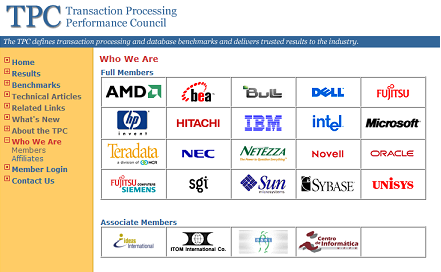
\includegraphics[width=0.8\linewidth]{figures/tpc/tpc_members.png}
\end{center}
\caption{Członkowie TPC~\cite{TPC1}}\label{rys:tpc_members}
\end{figure}
Organizacja ta przygotowuje specyfikacje testów służących do badania i porównywania wydajności m.~in.: 
systemów zarządzania bazami danych (\akronim{SZBD}, \english{DBMS}). Na podstawie tych specyfikacji tworzone są benchmarki, 
czyli narzędzia pomiaru wydajności, dla konkretnych DBMS. Z uzyskanych wyników publikowane są raporty 
umożliwiające porównanie wydajności różnych rozwiązań. Organizacja TPC skupia ekspertów z zakresu baz danych, reprezentujących
duże, znane przedsiębiorstwa (zob.~rys.~\ref{rys:tpc_members}). Niestety członkostwo nie jest darmowe~\cite{TPC1}:

\begin{quote}
Full Members of the TPC participate in all aspects of the TPC's work, including
development of benchmark standards and setting strategic direction. 
Full Membership costs $\$15\,000$ per calendar year.
\end{quote}

\noindent%
W związku z powyższym w grupie tej brakuje przedstawicieli rozwiązań niekomercyjnych jak
MySQL czy PostgreSQL.

Specyfikacje testów TPC różnią się między sobą zakresem badanych właściwości. 
Zakres ten dla konkretnej specyfikacji odpowiada właściwością konkretnego typu DBMS.
Poniżej wymieniono benchmarki TPC dotyczące baz danych.

\begin{description}
\item[TPC-A (OLTP) (1989)] 
TPC-A jest odmianą benchmarku debetowo-kredytowego OLTP (1985). Model bazy danych reprezentuje
w nim bank. Baza danych składa się z czterech typów rekordów: rachunek, kasjer, oddział, historia.
Miarą efektywności jest wydajność mierzona liczbą transakcji na jedną sekundę. 90\% transakcji powinno mieć czas
odpowiedzi 2 sekundy lub krótszy. Benchmark ten jest przestarzały. 

\item[TPC-B (\english{database stress test}) (sierpień 1990)]
W tym benchmarku nie ma użytkowników, linii komunikacyjnych czy terminali. Jest to test obciążeniowy,
dotyczący głównie operacji dyskowych. Benchmark ten nie jest testem OLTP i podobnie jak TPC-A jest przestarzały.

\item[TPC-C (OLTP) (lipiec 1992)]
Benchmark ten jest testem OLTP, bardziej złożonym od TPC-A. Występuje w nim mieszanka 5 różnych typów transakcji,
z których mierzy się czasy dla jednej, a pozostałe pełnia rolę szumu. Model bazy danych jest typową hurtownią składającą 
się z 9 relacji o określonej, skalowalnej liczbie rekordów i powiązań. Miarą efektywności jest tutaj liczba wykonanych 
transakcji typu ,,nowe zamówienie'' na minutę. Bliższe informacje odnośnie tego benchmarku znajdują się w dalszej części rozdziału.  

\item[TPC-D (kwiecień 1995)]
TPC-D reprezentuje szeroki zakres aplikacji wspomagania decyzji, które wymagają złożonych długotrwających zapytań,
na dużych skomplikowanych strukturach danych~\cite{TPC1}.

\item[TPC-H]
Benchmark ten jest kolejnym testem przeznaczonym dla systemów bazodanowych zorientowanych na wspomaganie decyzji,
w których występują duże, złożone struktury danych i duże, złożone zapytania. W przeciwieństwie do TPC-D, w benchmarku
tym podczas tego typu operacji wykonywane są równolegle pewne operacje modyfikujące dane.

\item[TPC-R] 
TPC-R jest benchmarkiem podobnym do TPC-H, lecz dodatkowo uwzględnia możliwość optymalizacji zapytań na podstawie
zaawansowanej wiedzy odnośnie zapytań.

\item[TPC-W]
Jest to benchmark transakcji dla aplikacji opartych o interfejs stron WWW. Test ten porusza wiele
cech charakterystycznych w tego typu systemach takich jak:
\begin{itemize}
    \item występowanie wielu sesji użytkowników,
    \item dynamiczne generowanie stron z jednoczesnym dostępem do bazy danych i jej uaktualnianiem,
    \item komunikacja w oparciu o protokół HTTP.
\end{itemize}
Miarą efektywności jest tutaj liczba interakcji ze stroną na sekundę. Wielokrotne interakcje ze stroną WWW
są wykorzystywane w celu symulacji rzeczywistej sprzedaży detalicznej. Każda interakcja jest przedmiotem
indywidualnych ograniczeń czasowych.

\item[TPC-App (\english{Application Server and Web Services Benchmark})]
TPC-App jest benchmarkiem serwerów aplikacji i technologii WebServices. Benchmark ten wykorzystuje w testach
komunikację opartą o dokumenty XML i protokół SOAP. Uwzględnia również wielosesyjność systemów oraz
dynamiczną konstrukcję odpowiedzi WebServices opartą o dostęp i modyfikację bazy danych. Baza danych składa się z
wielu tabel złożonych z dużej liczby kolumn, wierszy i powiązań. Od systemu wymaga się spełnienia właściwości 
\akronim{ACID}, zapewniających integralność transakcji. Miarą wydajności jest tutaj liczba obsłużonych
żądań.
\end{description}

Z powyższej listy specyfikacji wynika jeden istotny wniosek -- nie istnieje 
jeden uniwersalny benchmark umożliwiający badanie wydajności całej gamy istniejących
systemów zarządzania bazami danych. Również budowane rozwiązanie jest ukierunkowane
na badanie cech SZBD głównie typu OLTP. Dlatego też w kolejnym rozdziale zostanie
przybliżona specyfikacja benchmarku TPC-C.

\section{Benchmark TPC-C}

Benchmark TPC-C jest specyfikacją modelu pomiarowego dla systemów zarządzania bazami danych. 
Model ten opisuje strukturę bazy danych zgodnej z OLTP, jak i metodologię dokonywania pomiarów.
Specyfikacja ta jest niezależna od konkretnego DBMS. TPC-C nie jest zatem narzędziem pomiaru wydajności,
jest raczej specyfikacją budowy i użytkowania takiego narzędzia dla konkretnego DBMS. Specyfikacja 
ta rozwijana jest od połowy 1992 roku przez organizację TPC (aktualna wersja specyfikacji to wersja 5.6).

Warto też w tym miejscu wymienić cechy charakterystyczne OLTP, są to:
\begin{itemize}
\item proste operacje SQL typu select, insert, update oraz delete,
\item duża liczba klientów i wielodostęp,
\item najważniejszym parametrem jest średni czas wykonania komendy sql,
\item współbieżność transakcji, rozwiązywanie konfliktów,
\item miliony transakcji.
\end{itemize}
A zatem pomiary dokonywane przez benchmarki OLTP wymagać będą tych cech.

Specyfikacja TPC-C zawiera opis bazy danych, dla której dokonywane mają być testy. Struktura
bazy nie może ulegać odstępstwom, w zależności od konkretnej implementacji benchmarku.
Opis ten zawiera zarówno omówienie relacji, powiązań między nimi, jak i populację bazy danych
przed rozpoczęciem testów (zob.~rys.~\ref{rys:tpc_db_structure} oraz rys.~\vref{rys:tpc_db_structure2}). 
W ramach populacji omówiona jest nie tylko liczba rekordów w poszczególnych relacjach 
w zależności od parametru skalującego, lecz również rozkład wartości 
poszczególnych atrybutów i ich cechy szczególne takie jak unikalność, możliwość
przyjmowania wartości pustych.

\begin{figure}[p]
\begin{center}
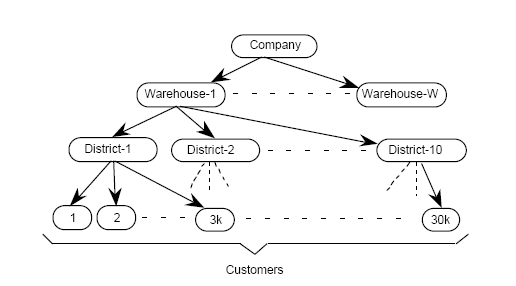
\includegraphics[width=\linewidth]{figures/tpc/tpc_db_structure.png}
\end{center}
\caption{Struktura bazy danych dla TPC-C~\cite{TPC1}}\label{rys:tpc_db_structure}
\end{figure}

\begin{figure}[p]
\begin{center}
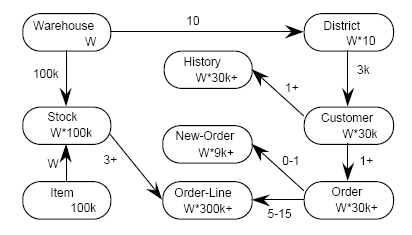
\includegraphics[width=\linewidth]{figures/tpc/tpc_db_structure2.png}
\end{center}
\caption{Struktura bazy danych dla TPC-C~\cite{TPC1}}\label{rys:tpc_db_structure2}
\end{figure}
\afterpage{\clearpage} % wymuś stronę rysunków po tej stronie.

TPC-C specyfikuje pięć typowych transakcji dla zaproponowanego modelu bazy danych.
To właśnie te transakcje, o określonej proprocji występowania, poddawane są testom. 
Warto zauważyć, że dla dowolnego schematu relacji zbiór wszystkich możliwych transakcji jest olbrzymi,
nie chodzi zatem o to by przetestować wszystkie te transakcje, lecz aby wybrać
do przetestowania najbardziej typowe -- te, z którymi mielibyśmy do czynienia
w bazie użytkowej. Ważnym elementem są scenariusze, które określają prawdopodobieństwo
wykonania operacji danego typu, po zakończeniu operacji innego typu. Omówione zostały również 
kwestie skalowalności populacji.

Dla każdej z 5 transakcji omówiono sposób generowania danych wejściowych,
profil jak i szczegółowe informacje dotyczące wymagań odnośnie wejścia/wyjścia 
terminali pomiarowych -- \akronim{RTE} (\english{Remote Terminal Emulator)}.

Rozdział 3 specyfikacji omawia właściwości jakie powinien spełniać system
podczas przeprowadzania pomiarów~\cite{TPC2}:

\begin{quote}
The ACID (Atomicity, Consistency, Isolation, and Durability) properties of 
transaction processing systems must be supported by the system under test 
during the running of this benchmark.
\end{quote}

Przyjrzymy się bliżej tym właściwościom:
\begin{itemize}
\item atomowość -- system poddawany testom musi gwarantować atomowość transakcji;
\item spójność -- wykonanie transakcji musi powodować przejście bazy danych z jednego stanu spójnego do innego;
\item izolacja -- poziom izolacji transakcji określany jest na podstawie występowania, bądź nie, 4 anomalii,
są nimi: ,,brudny zapis''(\english{Dirty Write}), ,,brudny odczyt''(\english{Dirty Read}), 
,,niepowtarzalny odczyt''(\english{Non-repeatable Read}) oraz ,,fantom''(\english{Phantom}). 
Sposób wyznaczenia poziomu izolacji w zależności od anomalii obrazuje tab.~\vref{tab:isol_tab}.
Dla każdej z 5 transakcji określono poziom izolacji, jaki musi zapewniać system poddawany testom;

\begin{table}[t]
\caption{Poziomy izolacji i anomalie.}\label{tab:isol_tab}
\scriptsize\centering%
\begin{tabular}{c c c c c}
\toprule
Poziom izolacji & \multicolumn{4}{c}{Anomalia} \\ \cmidrule{2-5}
                & Brudny zapis & Brudny odczyt & Niepowtarzalny odczyt & Fantom \\ \midrule
0 & Niemożliwy & Możliwy    & Możliwy   & Możliwy    \\
1 & Niemożliwy & Niemożliwy & Możliwy   & Możliwy    \\
2 & Niemożliwy & Niemożliwy & Niemożliwy& Możliwy    \\
3 & Niemożliwy & Niemożliwy & Niemożliwy& Niemożliwy \\
\bottomrule
\end{tabular}
\end{table}

\item trwałość -- testowany system musi zapewniać trwałość, oznacza to, że w przypadku wystąpienia
awarii, system musi umożliwiać odzyskanie ostatniego stanu spójnego bazy danych sprzed awarii.
\end{itemize}

Specyfikacja TPC-C opisuje również bardzo szczegółowo tworzenie wymaganych raportów.
Zestaw takich metryk po zakończeniu pomiarów powinien być przekazany wraz z wynikami do organizacji TPC-C.
Na rys.~\vref{rys:tpc_required_reporting1} przedstawiono przykładowy raport obrazujący
liczbę transakcji danego typu, w zależności od czasu ich odpowiedzi. Raport ten musi, między innymi, posiadać 
20 równej długości przedziałów na osi $X$, a także oś ta musi mieć długość równą 
4 krotnej długości przypadającej na 90\% transakcji. 

\begin{figure}[p]
\begin{center}
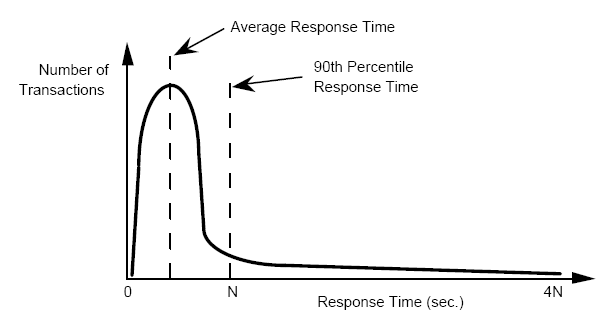
\includegraphics[width=\linewidth]{figures/tpc/tpc_required_reporting1.png}
\end{center}
\caption{Czas odpowiedzi (źródło:~\cite{TPC2}).}\label{rys:tpc_required_reporting1}
\end{figure}

\begin{figure}[p]
\begin{center}
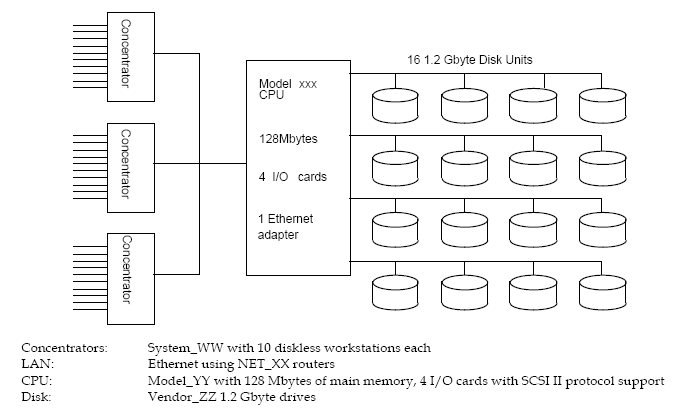
\includegraphics[width=\linewidth]{figures/tpc/tpc_full_disclosure1.png}
\end{center}
\caption{Przykładowy diagram połączeń\cite{TPC2}}\label{rys:tpc_full_disclosure1}
\end{figure}

Nierozerwalną częścią raportu z przeprowadzonych testów są również:
\begin{itemize}
\item Dokładny i szczegółowy opis środowiska, w którym przeprowadzono testy -- opis ten powinien uwzględniać szereg aspektów: 
parametry sprzętu komputerowego, jego liczba, sposób łączenia, sposób konfiguracji SZBD, parametry sieci, opis
systemu operacyjnego i niezbędnego oprogramowania. W tym celu można załączać wszelkiego rodzaju diagramy takie jak
np.~rys.~\vref{rys:tpc_full_disclosure1}.\afterpage{\clearpage}
\item Wycena systemu, w którym przeprowadzono testy -- w skład tej wyceny powinny wejść takie elementy jak sprzęt komputerowy, 
infrastruktura sieciowa, w tym urządzenia sieciowe, system operacyjny jak i inne niezbędne oprogramowanie, SZBD, 
zakup niezbędnych licencji itd. O dużej wadze przywiązywanej przez twórców do tego elementu
świadczyć może poświęcenie wycenie odrębnego rozdziału w specyfikacji.
\end{itemize}

Aby wyniki testów były ważne, tj.~uznane przez TPC, niezbędne jest również przejście pozytywnie
przez procedurę audytu przeprowadzaną przez niezależnych audytorów licencjonowanych
przez organizację TPC. Specyfikacja benchmarku TPC-C zawiera zatem listę kontrolną
na podstawie której przeprowadzany jest audyt, a także dokładny opis tej procedury.

Dopiero po spełnieniu tych wszystkich wymagań wyniki testu TPC-C mogą być opublikowane przez organizację TPC.
Wyniki takie służą do porównywania wydajności poszczególnych SZBD. Na rys.~\vref{rys:tpc_sample_results} 
przedstawiono przykładowe wyniki publikowane przez organizacje TPC. Jest to skrócona wersja wyników. 
Najważniejszymi wskaźnikami są tutaj \akronim{tpmC} (\english{transactions per minute}) 
-- liczba transakcji typu ,,nowe zamówienie'' wykonanych na minutę oraz \akronim{price/tpmC} czyli 
koszt podzielony przez liczbę tych transakcji na minutę.

\begin{figure}[htp]
\begin{center}
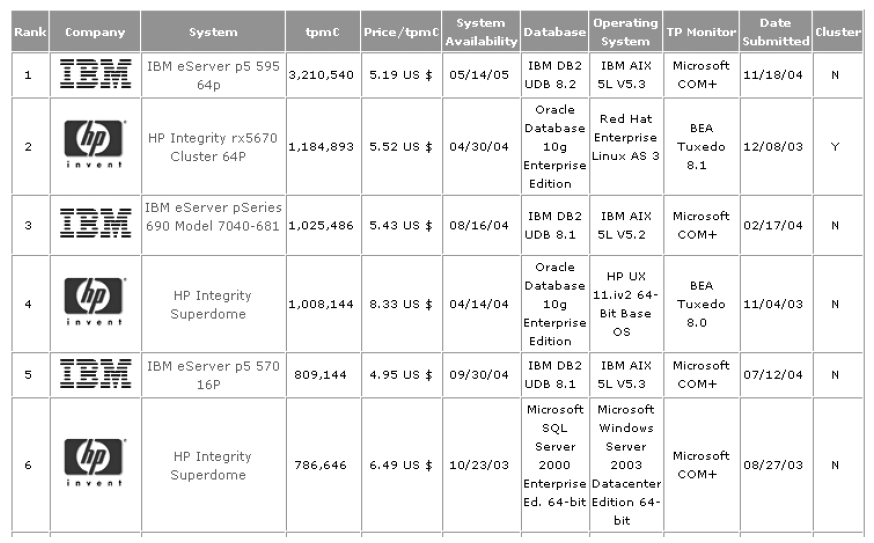
\includegraphics[width=\linewidth]{figures/tpc/tpc_sample_results.png}
\end{center}
\caption{Przykładowe wyniki TPC (źródło: \cite{TPC1}).}\label{rys:tpc_sample_results}
\end{figure}

W związku z tym, iż benchmark ten jest z reguły wykorzystywany przez twórców bazy danych,
gotowych ponieść duże nakłady finansowe, aby uzyskać w teście możliwie jak najlepsze rezultaty,
z punktu widzenia użytkownika najistotniejszym kryterium wydaje się być stosunek ceny zbudowanego systemu,
poddawanego testom, do liczby transakcji obsługiwanych przez ten system w jednostce czasu. 

\section{Podsumowanie}

Z powyższego opisu benchmarku TPC-C można wysnuć kilka istotnych wniosków:

\begin{itemize}
    \item TPC-C jest specyfikacją -- aby przeprowadzić testy wybranego SZBD należy zaimplementować 
    tą specyfikację dla niego.
    \item Niezmienną rzeczą w teście jest ustalony model bazy danych. W przypadku próby sprawdzenia,
    jak na konkretnym SZBD zachowuje się pod względem wydajności, inny model bazy danych, nie można
    posłużyć się tym benchmarkiem.
    \item Benchmark jest przeznaczony do opracowania raportów publikowanych przez TPC. Raporty te służą
    do porównywania nie tylko SZBD, ale całych platform bazodanowych.
\end{itemize}

W przeciwieństwie do powyższych cech, budowany w tej pracy benchmark ma charakteryzować się:
\begin{itemize}
    \item możliwością stworzenia własnych modeli bazy danych i obciążenia bazy danych,
    \item dostępnością predefiniowanych modeli baz danych,
    \item możliwością przeprowadzenia testów na więcej niż jednym SZBD (Oracle, PostgreSQL, MySQL),
    \item uniezależnieniem modelu bazy danych i obciążenia od konkretnego SZBD. 
\end{itemize}

W przeciwieństwie do TPC-C system testujący przygotowany w pracy ma spełniać głównie funkcje użytkowe, 
ze względu na swoją prostotę, ale i elastyczność ma być narzędziem, dostępnym dla zwykłego użytkownika.

